\documentclass[aspectratio=169,10pt]{beamer}

\usetheme[progressbar=frametitle,numbering=fraction,block=fill]{metropolis}
\usepackage{amsmath,amssymb,bm}
\usepackage{booktabs}
\usepackage{tikz}
\usetikzlibrary{calc,arrows.meta}

\newcommand{\R}{\mathbb{R}}
\newcommand{\w}{\mathbf{w}}
\newcommand{\x}{\mathbf{x}}

% ------------------------------------------------------------------
% TikZ styles and toy data
% Positive class: x1 + x2 >= 6, negative class: x1 + x2 <= 2.
% Best separating line: x1 + x2 = 4.
% ------------------------------------------------------------------
\definecolor{posc}{HTML}{C0392B}
\definecolor{negc}{HTML}{2471A3}
\definecolor{svc}{HTML}{E67E22}
\tikzset{
  ptpos/.style={circle,fill=posc,inner sep=0pt,minimum size=5pt},
  ptneg/.style={rectangle,fill=negc,inner sep=0pt,minimum size=5pt},
  sv/.style={circle,draw=svc,very thick,inner sep=0pt,minimum size=11pt},
}
\newcommand{\axes}{%
  \draw[->,gray] (-0.2,0) -- (6.3,0) node[below] {\scriptsize $x_1$};
  \draw[->,gray] (0,-0.2) -- (0,6.3) node[left] {\scriptsize $x_2$};
}
\newcommand{\posdata}{%
  \foreach \p in {(3,3),(4,2),(5,4),(4.5,3),(3.5,4.5),(5.5,2.2)} \node[ptpos] at \p {};
}
\newcommand{\negdata}{%
  \foreach \p in {(1,1),(0.5,1.5),(0.4,0.6),(1.2,0.3),(0.2,1.2)} \node[ptneg] at \p {};
}

% regression toy data: y = 0.5 x + 1 + noise
\tikzset{ptreg/.style={circle,fill=black!65,inner sep=0pt,minimum size=4.5pt}}
\newcommand{\regnoise}{0.3/0.3,0.8/-0.4,1.2/0.1,1.7/0.5,2.1/-0.2,2.6/-0.6,3.0/0.2,3.4/0.7,3.9/-0.3,4.3/0.1,4.8/-0.5,5.2/0.4,5.7/-0.1}

% SVR panel: #1 = epsilon, #2 = list of support vectors (x/noise)
\newcommand{\svrpanel}[2]{%
  \begin{tikzpicture}[scale=0.6]
    \draw[->,gray] (-0.2,0) -- (6.3,0) node[below] {\scriptsize $x_1$};
    \draw[->,gray] (0,-0.2) -- (0,5.2) node[left] {\scriptsize $y$};
    \fill[svc!14] (0,{1-#1}) -- (6,{4-#1}) -- (6,{4+#1}) -- (0,{1+#1}) -- cycle;
    \draw[svc!70!black,thick,dashed] (0,{1-#1}) -- (6,{4-#1});
    \draw[svc!70!black,thick,dashed] (0,{1+#1}) -- (6,{4+#1});
    \draw[very thick] (0,1) -- (6,4);
    \foreach \xx/\nn in \regnoise \node[ptreg] at (\xx,{0.5*\xx+1+\nn}) {};
    \foreach \xx/\nn in {#2} \node[sv] at (\xx,{0.5*\xx+1+\nn}) {};
    \draw[<->,thick] (6.15,4) -- (6.15,{4+#1}) node[midway,right,font=\scriptsize] {$\varepsilon$};
  \end{tikzpicture}}

% perturbation disks of radius 0.7 around every data point
\newcommand{\balls}[1]{%
  \foreach \p in {(3,3),(4,2),(5,4),(4.5,3),(3.5,4.5),(5.5,2.2),(1,1),(0.5,1.5),(0.4,0.6),(1.2,0.3),(0.2,1.2)}
    \fill[#1,opacity=0.18] \p circle (0.7);}

% ------------------------------------------------------------------
\title{Support Vector Machines}
\subtitle{CSS 324: Introduction to Machine Learning}
\author{}
\date{}

\begin{document}

\maketitle

% ==================================================================
\begin{frame}{Linear separability}
\begin{columns}[c]
\column{0.46\textwidth}
\centering
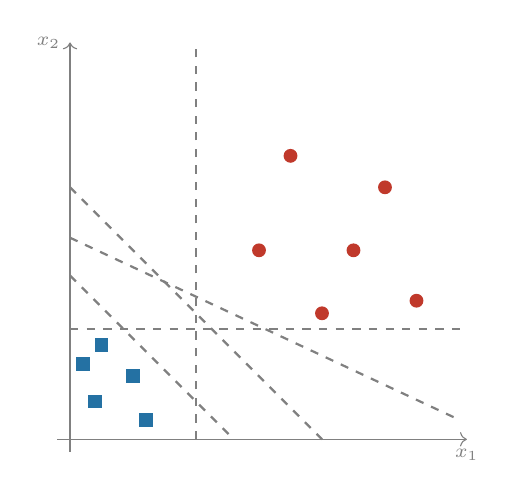
\begin{tikzpicture}[scale=0.8]
  \axes
  \begin{scope}
    \clip (-0.2,-0.2) rectangle (6.3,6.3);
    % candidate separating lines
    \draw[thick,gray,dashed] (2,0) -- (2,6.2);
    \draw[thick,gray,dashed] (0,1.75) -- (6.2,1.75);
    \draw[thick,gray,dashed] (0,2.6) -- (2.6,0);
    \draw[thick,gray,dashed] (0,3.2) -- (6.2,0.3);
    \draw[thick,gray,dashed] (0,4) -- (4,0);
  \end{scope}
  \posdata \negdata
\end{tikzpicture}
\column{0.52\textwidth}
\begin{itemize}
  \item A \textbf{linear classifier} separates two classes with a line. In $n$ dimensions the line becomes a \textbf{hyperplane}.
  \item The data are \textbf{linearly separable} if at least one such line separates the classes perfectly.
  \item In that case there are \emph{infinitely many} separating lines (gray dashed). Each one classifies the training set perfectly.
  \item \alert{Question:} which separating line should we choose?
\end{itemize}
\end{columns}
\end{frame}

% ==================================================================
\begin{frame}{The SVM idea: the widest street}
\begin{columns}[c]
\column{0.46\textwidth}
\centering
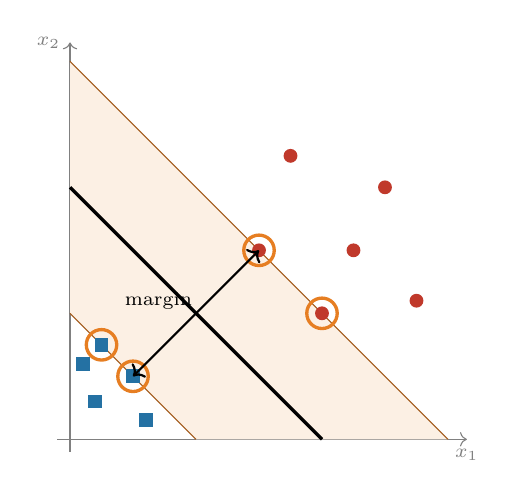
\begin{tikzpicture}[scale=0.8]
  \axes
  \begin{scope}
    \clip (-0.2,-0.2) rectangle (6.3,6.3);
    % margin "street" of the best line
    \fill[svc!12] (0,2) -- (2,0) -- (6,0) -- (0,6) -- cycle;
    \draw[svc!70!black,thin] (0,6) -- (6,0);
    \draw[svc!70!black,thin] (0,2) -- (2,0);
    % best separating line
    \draw[very thick] (0,4) -- (4,0);
  \end{scope}
  \posdata \negdata
  \foreach \p in {(3,3),(4,2),(1,1),(0.5,1.5)} \node[sv] at \p {};
  \draw[<->,thick] (1,1) -- (3,3) node[midway,above left,font=\scriptsize,inner sep=1pt] {margin};
\end{tikzpicture}
\column{0.52\textwidth}
\begin{itemize}
  \item A line close to the training points is fragile: a small change in the data can flip a prediction.
  \item \alert{SVM idea:} choose the line that stays \emph{as far as possible} from the closest points of both classes. That line has the widest ``street'' (\textbf{margin}) between the classes.
  \item The closest points (circled) are the \textbf{support vectors}. They alone determine the line.
  \item This approach is called \textbf{large margin classification}.
\end{itemize}
\end{columns}
\end{frame}

% ==================================================================
\begin{frame}{Decision function and prediction}
For an instance $\x = (x_1,\dots,x_n)^\top \in \R^n$, a linear SVM with weight vector $\w\in\R^n$ and bias $b\in\R$ computes the \textbf{decision function}
\[
  h(\x) \;=\; \w^\top\x + b \;=\; w_1x_1 + w_2x_2 + \cdots + w_nx_n + b .
\]

\begin{block}{Linear SVM classifier prediction}
\[
  \hat y \;=\;
  \begin{cases}
    0 & \text{if } \w^\top\x + b < 0,\\[2pt]
    1 & \text{if } \w^\top\x + b \ge 0.
  \end{cases}
\]
\end{block}

\begin{itemize}
  \item A nonnegative result predicts the positive class (1). A negative result predicts the negative class (0).
  \item The \textbf{decision boundary} $\{\x\in\R^n : \w^\top\x + b = 0\}$ is a line when $n=2$ and a hyperplane in general.
  \item \textbf{Training} a linear SVM means finding the $\w$ and $b$ that give the widest margin.
\end{itemize}
\end{frame}

% ==================================================================
\begin{frame}{The margin}
\begin{columns}[c]
\column{0.46\textwidth}
\centering
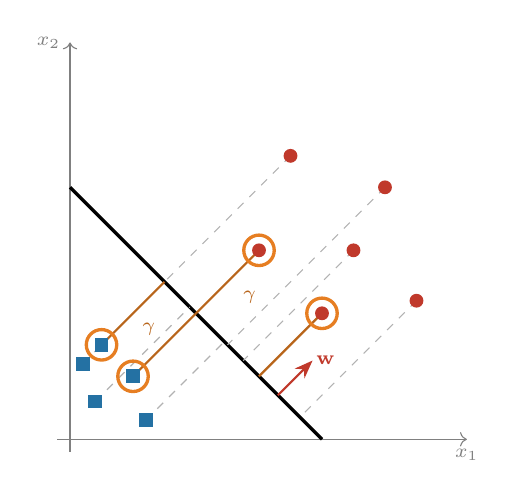
\begin{tikzpicture}[scale=0.8]
  \axes
  \begin{scope}
    \clip (-0.2,-0.2) rectangle (6.3,6.3);
    \draw[very thick] (0,4) -- (4,0);
  \end{scope}
  % distances of non-closest points (feet on x1 + x2 = 4)
  \foreach \a/\b in {5/4, 4.5/3, 3.5/4.5, 5.5/2.2, 0.4/0.6, 1.2/0.3, 0.2/1.2}
    \draw[gray!60,thin,dashed] (\a,\b) -- ({\a-(\a+\b-4)/2},{\b-(\a+\b-4)/2});
  % distances of the closest points
  \foreach \a/\b in {3/3, 4/2, 1/1, 0.5/1.5}
    \draw[svc!80!black,thick] (\a,\b) -- ({\a-(\a+\b-4)/2},{\b-(\a+\b-4)/2});
  \posdata \negdata
  \foreach \p in {(3,3),(4,2),(1,1),(0.5,1.5)} \node[sv] at \p {};
  \node[font=\scriptsize,svc!80!black] at (2.85,2.25) {$\gamma$};
  \node[font=\scriptsize,svc!80!black] at (1.25,1.75) {$\gamma$};
  \draw[-{Stealth},thick,posc] (3.3,0.7) -- (3.85,1.25) node[right,font=\scriptsize,inner sep=1pt] {$\w$};
\end{tikzpicture}
\column{0.52\textwidth}\small
\begin{block}{Distance from a point to the hyperplane}
\[
  d_i \;=\; \frac{|\w^\top\x_i + b|}{\lVert\w\rVert}
\]
\end{block}
\begin{block}{Margin of a separating hyperplane}
\[
  \gamma(\w,b) \;=\; \min_{i=1,\dots,m}\ \frac{|\w^\top\x_i + b|}{\lVert\w\rVert}
\]
\end{block}
\begin{itemize}
  \item The margin is the distance to the \emph{closest} training point. The width of the street is $2\gamma$.
  \item $\w$ is perpendicular to the boundary. Dividing by $\lVert\w\rVert$ turns $\w^\top\x+b$ into a distance.
  \item \alert{SVM:} among all separating hyperplanes, choose the one with the \textbf{largest} $\gamma$.
\end{itemize}
\end{columns}
\end{frame}

% ==================================================================
\begin{frame}{Why a large margin? Robustness to noise}
\begin{columns}[T]
\column{0.5\textwidth}
\centering
\textbf{Small margin}\\[3pt]
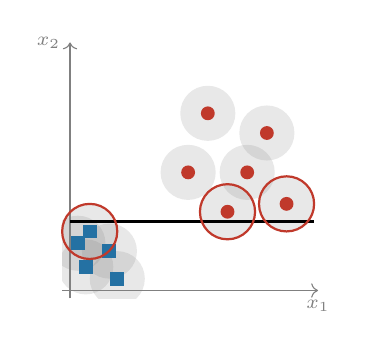
\begin{tikzpicture}[scale=0.5]
  \axes
  \begin{scope}
    \clip (-0.2,-0.2) rectangle (6.3,6.3);
    \balls{gray}
    \draw[very thick] (0,1.75) -- (6.2,1.75);
  \end{scope}
  \posdata \negdata
  \foreach \p in {(4,2),(5.5,2.2),(0.5,1.5)} \draw[posc,thick] \p circle (0.7);
\end{tikzpicture}
\column{0.5\textwidth}
\centering
\textbf{Large margin}\\[3pt]
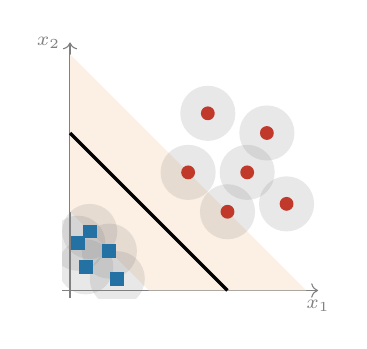
\begin{tikzpicture}[scale=0.5]
  \axes
  \begin{scope}
    \clip (-0.2,-0.2) rectangle (6.3,6.3);
    \fill[svc!12] (0,2) -- (2,0) -- (6,0) -- (0,6) -- cycle;
    \balls{gray}
    \draw[very thick] (0,4) -- (4,0);
  \end{scope}
  \posdata \negdata
\end{tikzpicture}
\end{columns}
\vspace{4pt}
\small
\begin{itemize}
  \item New data are noisy versions of the training data. The disks show a perturbation of radius $r$ around each point.
  \item \textbf{Left:} the boundary cuts through several disks (red), so a small perturbation of those points flips their predicted class.
  \item \textbf{Right:} every disk lies on one side. A perturbation smaller than $\gamma$ \emph{never} changes the prediction.
\end{itemize}
\end{frame}

% ==================================================================
\begin{frame}{Why is just a separating line not enough?}
\small
\begin{enumerate}
  \item \textbf{Training error cannot decide.} Every separating line has zero training error, yet they disagree on new points. For example, $\x=(2.5,\,1.2)$ is positive for the line $x_1=2$ but negative for $x_1+x_2=4$. We need an extra criterion.
  \item \textbf{Robustness.} A line close to training points is sensitive to noise and measurement errors. A large margin gives a ``safety zone'' of radius $\gamma$ around every training point.
  \item \textbf{Better generalization.} Few lines fit through a wide street, so large-margin classifiers are a \emph{simpler} model class that overfits less.
  \item \textbf{A unique, well-defined answer.} The maximum-margin line is unique and depends only on the support vectors. Points far from the street do not affect it.
\end{enumerate}
\begin{alertblock}{Bottom line}
Separating the training data is the \emph{minimum} requirement. Among all separating lines, the SVM chooses the most \emph{confident} one: the line with the largest margin.
\end{alertblock}
\end{frame}

% ==================================================================
\begin{frame}{From maximum margin to an optimization problem}
\begin{columns}[c]
\column{0.40\textwidth}
\centering
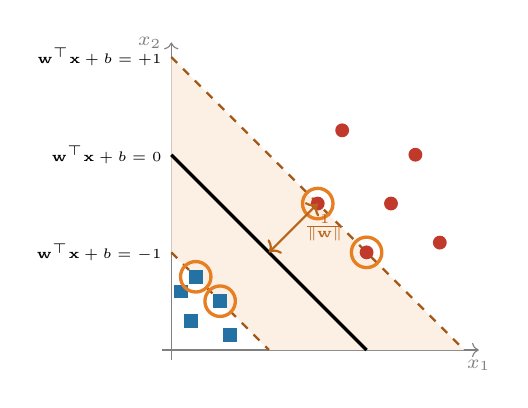
\begin{tikzpicture}[scale=0.62]
  \axes
  \begin{scope}
    \clip (-0.2,-0.2) rectangle (6.3,6.3);
    \fill[svc!12] (0,2) -- (2,0) -- (6,0) -- (0,6) -- cycle;
    \draw[svc!70!black,thick,dashed] (0,6) -- (6,0);
    \draw[svc!70!black,thick,dashed] (0,2) -- (2,0);
    \draw[very thick] (0,4) -- (4,0);
  \end{scope}
  \posdata \negdata
  \foreach \p in {(3,3),(4,2),(1,1),(0.5,1.5)} \node[sv] at \p {};
  \node[font=\tiny,left] at (0,6) {$\w^\top\x+b=+1$};
  \node[font=\tiny,left] at (0,4) {$\w^\top\x+b=0$};
  \node[font=\tiny,left] at (0,2) {$\w^\top\x+b=-1$};
  \draw[<->,thick,svc!80!black] (2,2) -- (3,3) node[midway,right,font=\scriptsize] {$\frac{1}{\lVert\w\rVert}$};
\end{tikzpicture}
\column{0.58\textwidth}
\small
Encode the labels as $t^{(i)} = +1$ if $y^{(i)}=1$ and $t^{(i)}=-1$ if $y^{(i)}=0$. Then instance $i$ is classified correctly iff $t^{(i)}(\w^\top\x^{(i)}+b) > 0$.

\vspace{4pt}
\textbf{Step 1: goal.} Maximize the margin
\[
  \max_{\w,b}\ \min_{i}\ \frac{t^{(i)}(\w^\top\x^{(i)}+b)}{\lVert\w\rVert}.
\]
\textbf{Step 2: fix the scale.} $(\w,b)$ and $(c\w,cb)$ with $c>0$ give the \emph{same} line. So we may choose the scale such that the closest points satisfy $t^{(i)}(\w^\top\x^{(i)}+b)=1$. Then
\[
  \gamma = \frac{1}{\lVert\w\rVert}, \qquad \text{street width} = \frac{2}{\lVert\w\rVert}.
\]
\textbf{Step 3: simplify.} Maximizing $\frac{1}{\lVert\w\rVert}$ is the same as minimizing $\tfrac12\lVert\w\rVert^2=\tfrac12\w^\top\w$, which is smooth and convex.
\end{columns}
\end{frame}

% ==================================================================
\begin{frame}{Hard margin linear SVM}
\begin{alertblock}{Hard margin linear SVM classifier objective}
\[
  \underset{\w,\,b}{\text{minimize}}\quad \frac12\,\w^\top\w
  \qquad\text{subject to}\qquad
  t^{(i)}\big(\w^\top\x^{(i)} + b\big) \;\ge\; 1 \quad\text{for } i=1,2,\dots,m
\]
\end{alertblock}
\begin{itemize}
  \item \textbf{Objective} $\tfrac12\w^\top\w$: a small $\lVert\w\rVert$ means a \emph{wide} street, since the width is $2/\lVert\w\rVert$.
  \item \textbf{Constraints}: every instance lies on the correct side \emph{and outside the street}. ``Hard'' means no violations are allowed.
  \item \textbf{Support vectors} are the instances with $t^{(i)}(\w^\top\x^{(i)}+b)=1$. They sit exactly on the edges of the street.
  \item This is a \textbf{convex quadratic program (QP)}: a quadratic objective with linear constraints. For linearly separable data it has a \emph{unique} solution, which standard QP solvers can find.
  \item \alert{Limitation:} if the data are \textbf{not} linearly separable, the problem has no solution. A single outlier can also make the margin very narrow.
\end{itemize}
\end{frame}

% ==================================================================
\begin{frame}{Soft margin classification: why?}
\begin{columns}[T]
\column{0.5\textwidth}
\centering
\textbf{Not linearly separable}\\[3pt]
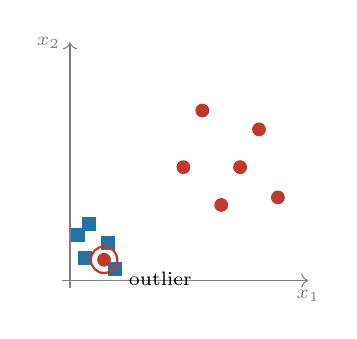
\begin{tikzpicture}[scale=0.48]
  \axes
  \posdata \negdata
  \node[ptpos] at (0.9,0.55) {};
  \draw[posc,thick] (0.9,0.55) circle (0.35);
  \node[font=\scriptsize,right] at (1.3,0.05) {outlier};
\end{tikzpicture}\\
\scriptsize No line separates the classes, so the hard margin problem has \emph{no solution}.
\column{0.5\textwidth}
\centering
\textbf{Outlier squeezes the margin}\\[3pt]
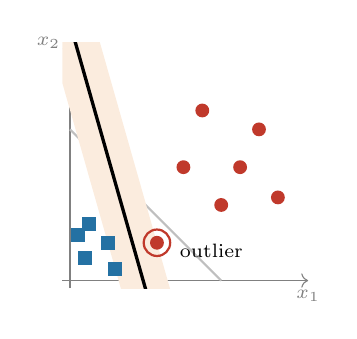
\begin{tikzpicture}[scale=0.48]
  \axes
  \begin{scope}
    \clip (-0.2,-0.2) rectangle (6.3,6.3);
    \draw[gray!50,thick] (0,4) -- (4,0);
    \coordinate (m) at (1.699,0.829);
    \coordinate (d) at (-0.274,0.962);
    \fill[svc!15] ($(2.3,1.0)-8*(d)$) -- ($(2.3,1.0)+8*(d)$) -- ($(1.098,0.657)+8*(d)$) -- ($(1.098,0.657)-8*(d)$) -- cycle;
    \draw[very thick] ($(m)-8*(d)$) -- ($(m)+8*(d)$);
  \end{scope}
  \posdata \negdata
  \node[ptpos] at (2.3,1.0) {};
  \draw[posc,thick] (2.3,1.0) circle (0.35);
  \node[font=\scriptsize,right] at (2.65,0.8) {outlier};
\end{tikzpicture}\\
\scriptsize The hard margin solution exists but is very narrow. It will likely generalize poorly.
\end{columns}
\vspace{6pt}
\small
\begin{itemize}
  \item The hard margin SVM is \textbf{sensitive to outliers} and works \textbf{only} for linearly separable data.
  \item \alert{Soft margin idea:} find a good balance between keeping the street \emph{as wide as possible} and limiting the \textbf{margin violations}, i.e.\ instances that end up inside the street or even on the wrong side.
\end{itemize}
\end{frame}

% ==================================================================
\begin{frame}{Slack variables}
\begin{columns}[c]
\column{0.44\textwidth}
\centering
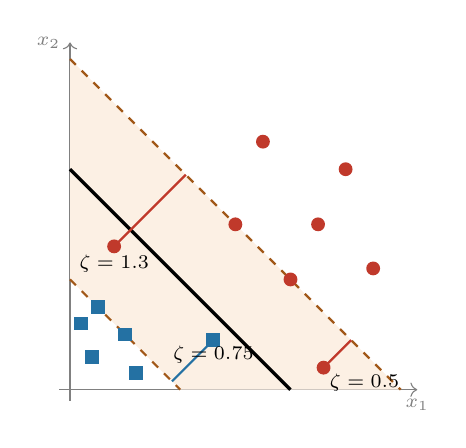
\begin{tikzpicture}[scale=0.7]
  \axes
  \begin{scope}
    \clip (-0.2,-0.2) rectangle (6.3,6.3);
    \fill[svc!12] (0,2) -- (2,0) -- (6,0) -- (0,6) -- cycle;
    \draw[svc!70!black,thick,dashed] (0,6) -- (6,0);
    \draw[svc!70!black,thick,dashed] (0,2) -- (2,0);
    \draw[very thick] (0,4) -- (4,0);
  \end{scope}
  \posdata \negdata
  % violators: slack drawn to their own margin line
  \draw[posc,thick] (4.6,0.4) -- (5.1,0.9);
  \draw[posc,thick] (0.8,2.6) -- (2.1,3.9);
  \draw[negc,thick] (2.6,0.9) -- (1.85,0.15);
  \node[ptpos] at (4.6,0.4) {};
  \node[ptpos] at (0.8,2.6) {};
  \node[ptneg] at (2.6,0.9) {};
  \node[font=\scriptsize,below right,inner sep=2pt] at (4.6,0.4) {$\zeta=0.5$};
  \node[font=\scriptsize,below,inner sep=3pt] at (0.8,2.6) {$\zeta=1.3$};
  \node[font=\scriptsize,below,inner sep=2pt] at (2.6,0.9) {$\zeta=0.75$};
\end{tikzpicture}
\column{0.54\textwidth}
\small
For each instance introduce a \textbf{slack variable} $\zeta^{(i)}\ge 0$ that measures how much it violates the margin, and relax the constraint to
\[
  t^{(i)}\big(\w^\top\x^{(i)}+b\big) \;\ge\; 1-\zeta^{(i)} .
\]
\begin{itemize}
  \item $\zeta^{(i)}=0$: on or outside the street, correct side. No violation.
  \item $0<\zeta^{(i)}\le 1$: inside the street but still correctly classified.
  \item $\zeta^{(i)}>1$: on the wrong side of the boundary, i.e.\ \textbf{misclassified}.
\end{itemize}
The smallest valid slack is
\[
  \zeta^{(i)} = \max\!\big(0,\ 1-t^{(i)}(\w^\top\x^{(i)}+b)\big).
\]
\end{columns}
\end{frame}

% ==================================================================
\begin{frame}{Soft margin linear SVM}
\begin{alertblock}{Soft margin linear SVM classifier objective}
\[
  \underset{\w,\,b,\,\bm{\zeta}}{\text{minimize}}\quad \frac12\,\w^\top\w \;+\; C\sum_{i=1}^{m}\zeta^{(i)}
  \qquad\text{subject to}\qquad
  \begin{aligned}
    & t^{(i)}\big(\w^\top\x^{(i)} + b\big) \ge 1-\zeta^{(i)}\\
    & \zeta^{(i)}\ge 0
  \end{aligned}
  \quad \forall i
\]
\end{alertblock}
\begin{itemize}
  \item Two \textbf{conflicting objectives}:
  \begin{itemize}
    \item $\tfrac12\w^\top\w$ small $\Rightarrow$ wide street;
    \item $\sum_i\zeta^{(i)}$ small $\Rightarrow$ few and small margin violations.
  \end{itemize}
  \item The hyperparameter $C>0$ sets the trade-off between them.
  \item The problem is still a \textbf{convex QP}, and it \emph{always} has a solution (take $\zeta^{(i)}$ large enough), even for data that are not linearly separable.
  \item As $C\to\infty$, violations become infinitely expensive and we recover the \textbf{hard margin} SVM.
\end{itemize}
\end{frame}

% ==================================================================
\begin{frame}{The hyperparameter $C$}
\begin{columns}[T]
\column{0.5\textwidth}
\centering
\textbf{Small $C$} (e.g.\ $C=0.1$)\\[3pt]
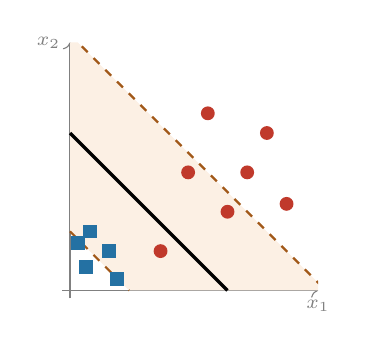
\begin{tikzpicture}[scale=0.5]
  \axes
  \begin{scope}
    \clip (-0.2,-0.2) rectangle (6.3,6.3);
    \fill[svc!12] (0,1.5) -- (1.5,0) -- (6.3,0) -- (6.3,0.2) -- (0.2,6.3) -- (0,6.3) -- cycle;
    \draw[svc!70!black,thick,dashed] (0,6.5) -- (6.5,0);
    \draw[svc!70!black,thick,dashed] (0,1.5) -- (1.5,0);
    \draw[very thick] (0,4) -- (4,0);
  \end{scope}
  \posdata \negdata
  \node[ptpos] at (2.3,1.0) {};
\end{tikzpicture}\\
\scriptsize Wide street, more margin violations.\\ Lower variance, may \emph{underfit}.
\column{0.5\textwidth}
\centering
\textbf{Large $C$} (e.g.\ $C=100$)\\[3pt]
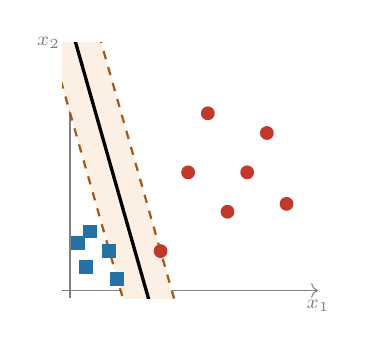
\begin{tikzpicture}[scale=0.5]
  \axes
  \begin{scope}
    \clip (-0.2,-0.2) rectangle (6.3,6.3);
    \coordinate (m) at (1.699,0.829);
    \coordinate (d) at (-0.274,0.962);
    \fill[svc!12] ($(2.3,1.0)-8*(d)$) -- ($(2.3,1.0)+8*(d)$) -- ($(1.098,0.657)+8*(d)$) -- ($(1.098,0.657)-8*(d)$) -- cycle;
    \draw[svc!70!black,thick,dashed] ($(2.3,1.0)-8*(d)$) -- ($(2.3,1.0)+8*(d)$);
    \draw[svc!70!black,thick,dashed] ($(1.098,0.657)-8*(d)$) -- ($(1.098,0.657)+8*(d)$);
    \draw[very thick] ($(m)-8*(d)$) -- ($(m)+8*(d)$);
  \end{scope}
  \posdata \negdata
  \node[ptpos] at (2.3,1.0) {};
\end{tikzpicture}\\
\scriptsize Narrow street, few or no violations.\\ Fits the outlier, may \emph{overfit}.
\end{columns}
\vspace{6pt}
\small
\begin{itemize}
  \item The model with small $C$ is likely to generalize better here, even though it makes more violations on the training set.
  \item \alert{Rule of thumb:} if your SVM model is overfitting, try \textbf{reducing} $C$. Tune $C$ with cross-validation.
\end{itemize}
\end{frame}

% ==================================================================
\begin{frame}{Equivalent view: the hinge loss}
\begin{columns}[c]
\column{0.42\textwidth}
\centering
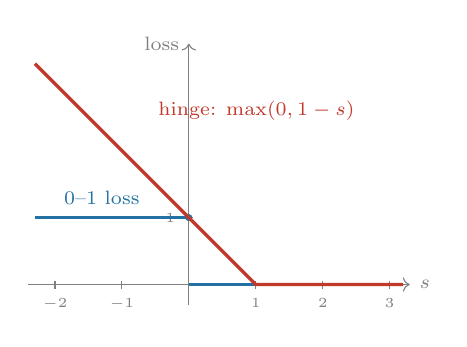
\begin{tikzpicture}[scale=0.85]
  \draw[->,gray] (-2.4,0) -- (3.3,0) node[right] {\scriptsize $s$};
  \draw[->,gray] (0,-0.3) -- (0,3.6) node[left] {\scriptsize loss};
  \foreach \xx in {-2,-1,1,2,3} \draw[gray] (\xx,0.06) -- (\xx,-0.06) node[below,font=\tiny] {$\xx$};
  \draw[gray] (0.06,1) -- (-0.06,1) node[left,font=\tiny] {$1$};
  % 0-1 loss
  \draw[negc,very thick] (-2.3,1) -- (0,1);
  \draw[negc,very thick] (0,0) -- (3.2,0);
  \fill[negc] (0,1) circle (1.5pt);
  % hinge loss
  \draw[posc,very thick] (-2.3,3.3) -- (1,0) -- (3.2,0);
  \node[posc,font=\scriptsize,right] at (-0.6,2.6) {hinge: $\max(0,1-s)$};
  \node[negc,font=\scriptsize,above] at (-1.3,1.05) {0--1 loss};
\end{tikzpicture}
\column{0.56\textwidth}
\small
Substituting the optimal slack $\zeta^{(i)}=\max\big(0,1-t^{(i)}(\w^\top\x^{(i)}+b)\big)$ gives an \textbf{unconstrained} problem:
\[
  J(\w,b) = \frac12\w^\top\w \;+\; C\sum_{i=1}^{m}\max\!\Big(0,\ 1-t^{(i)}\big(\w^\top\x^{(i)}+b\big)\Big).
\]
\begin{itemize}
  \item With $s=t^{(i)}(\w^\top\x^{(i)}+b)$, the loss is $0$ for instances off the street on the correct side ($s\ge1$), and grows \emph{linearly} with the violation.
  \item The hinge loss is a convex upper bound on the 0--1 (misclassification) loss.
  \item $J$ can be minimized by (sub)gradient descent, e.g.\ \texttt{SGDClassifier(loss="hinge")} in Scikit-Learn.
\end{itemize}
\end{columns}
\end{frame}

% ==================================================================
\begin{frame}{Nonlinear data: adding features}
\begin{columns}[c]
\column{0.5\textwidth}
\centering
\textbf{Original feature $x_1$}\\[6pt]
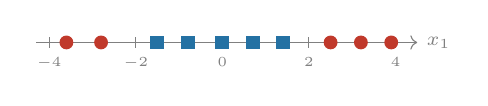
\begin{tikzpicture}[x=0.55cm,y=0.55cm]
  \draw[->,gray] (-4.3,0) -- (4.5,0) node[right] {\scriptsize $x_1$};
  \foreach \xx in {-4,-2,0,2,4} \draw[gray] (\xx,0.12) -- (\xx,-0.12) node[below,font=\tiny] {$\xx$};
  \foreach \xx in {-1.5,-0.8,0,0.7,1.4} \node[ptneg] at (\xx,0) {};
  \foreach \xx in {-3.6,-2.8,2.5,3.2,3.9} \node[ptpos] at (\xx,0) {};
\end{tikzpicture}\\[8pt]
\scriptsize No single threshold on $x_1$ separates the classes.
\column{0.5\textwidth}
\centering
\textbf{Add feature $x_2 = x_1^2$}\\[3pt]
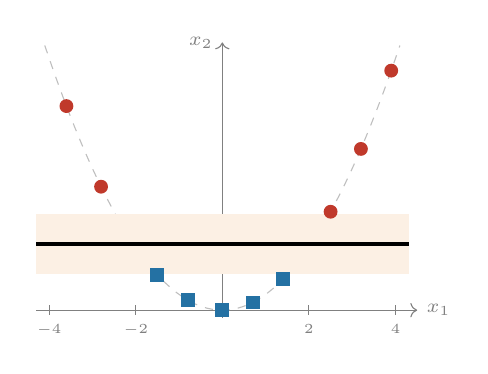
\begin{tikzpicture}[x=0.55cm,y=0.2cm]
  \draw[->,gray] (-4.3,0) -- (4.5,0) node[right] {\scriptsize $x_1$};
  \draw[->,gray] (0,-0.5) -- (0,17) node[left] {\scriptsize $x_2$};
  \foreach \xx in {-4,-2,2,4} \draw[gray] (\xx,0.3) -- (\xx,-0.3) node[below,font=\tiny] {$\xx$};
  \draw[gray!50,dashed,domain=-4.1:4.1,samples=60] plot (\x,{\x*\x});
  \fill[svc!12] (-4.3,2.3) rectangle (4.3,6.1);
  \draw[very thick] (-4.3,4.2) -- (4.3,4.2);
  \foreach \xx in {-1.5,-0.8,0,0.7,1.4} \node[ptneg] at (\xx,{\xx*\xx}) {};
  \foreach \xx in {-3.6,-2.8,2.5,3.2,3.9} \node[ptpos] at (\xx,{\xx*\xx}) {};
\end{tikzpicture}\\
\scriptsize Now the data are \textbf{linearly separable}.
\end{columns}
\vspace{6pt}
\small
\begin{itemize}
  \item \textbf{Idea:} map each instance to a higher-dimensional feature space, $\x\mapsto\phi(\x)$, and train a \emph{linear} SVM there. A line in feature space is a \emph{curve} in the original space.
  \item In Scikit-Learn: \texttt{PolynomialFeatures(degree=3)} followed by \texttt{LinearSVC}.
\end{itemize}
\end{frame}

% ==================================================================
\begin{frame}{The problem with explicit features}
\small
\begin{itemize}
  \item Polynomial features of degree $d$ in $n$ original features give $\binom{n+d}{d}$ new features:
\end{itemize}
\begin{center}
\begin{tabular}{@{}rrr@{}}
\toprule
$n$ & degree $d$ & number of features \\
\midrule
2 & 3 & 10 \\
10 & 3 & 286 \\
100 & 3 & 176{,}851 \\
1000 & 3 & $\approx 1.7\times 10^{8}$ \\
\bottomrule
\end{tabular}
\end{center}
\begin{itemize}
  \item A low degree cannot fit complex data. A high degree creates a \textbf{combinatorial explosion} of features, which makes the model too slow to train and to use.
  \item For some useful feature maps (e.g.\ the Gaussian RBF below), $\phi(\x)$ is even \textbf{infinite-dimensional}.
\end{itemize}
\vspace{4pt}
\alert{Question:} can we get the benefit of a high-dimensional $\phi$ \emph{without} ever computing $\phi(\x)$? \textbf{Yes: the kernel trick.}
\end{frame}

% ==================================================================
\begin{frame}{The dual problem: data only through dot products}
\small
Using Lagrange duality, the soft margin SVM can be rewritten as an equivalent \textbf{dual problem} in variables $\alpha^{(i)}$. We state it without derivation:
\begin{alertblock}{Dual form of the linear SVM objective}
\[
  \underset{\bm\alpha}{\text{minimize}}\quad
  \frac12\sum_{i=1}^{m}\sum_{j=1}^{m}\alpha^{(i)}\alpha^{(j)}t^{(i)}t^{(j)}\,
  \underbrace{{\x^{(i)}}^\top\x^{(j)}}_{\text{dot product}}
  \;-\;\sum_{i=1}^{m}\alpha^{(i)}
  \qquad\text{subject to}\quad
  \begin{aligned}
    & 0\le\alpha^{(i)}\le C\\
    & \textstyle\sum_{i}\alpha^{(i)}t^{(i)}=0
  \end{aligned}
\]
\end{alertblock}
From the solution $\hat{\bm\alpha}$:
\[
  \hat\w = \sum_{i=1}^{m}\hat\alpha^{(i)}t^{(i)}\x^{(i)},
  \qquad
  h(\x) = \hat\w^\top\x + \hat b = \sum_{\hat\alpha^{(i)}>0}\hat\alpha^{(i)}t^{(i)}\,{\x^{(i)}}^\top\x \;+\; \hat b .
\]
\begin{itemize}
  \item $\hat\alpha^{(i)}>0$ \emph{only} for the support vectors, so the sum is over a few instances.
  \item \alert{Key observation:} both training and prediction use the data \textbf{only through dot products} ${\x^{(i)}}^\top\x^{(j)}$.
\end{itemize}
\end{frame}

% ==================================================================
\begin{frame}{The kernel trick}
\small
\textbf{Example.} The 2nd-degree polynomial map for $\x=(x_1,x_2)$:
\[
  \phi(\x) = \big(x_1^2,\ \sqrt2\,x_1x_2,\ x_2^2\big)^\top \in\R^3 .
\]
For two vectors $\mathbf a,\mathbf b\in\R^2$:
\[
  \phi(\mathbf a)^\top\phi(\mathbf b)
  = a_1^2b_1^2 + 2a_1b_1a_2b_2 + a_2^2b_2^2
  = (a_1b_1+a_2b_2)^2
  = \big(\mathbf a^\top\mathbf b\big)^2 .
\]
The dot product in feature space is computed \textbf{in the original space}, without computing $\phi$.

\begin{block}{Kernel}
A \textbf{kernel} is a function $K(\mathbf a,\mathbf b) = \phi(\mathbf a)^\top\phi(\mathbf b)$ that computes the dot product of the transformed vectors from $\mathbf a$ and $\mathbf b$ alone.
\end{block}
\begin{itemize}
  \item \alert{Kernel trick:} in the dual problem and in the prediction, replace every ${\x^{(i)}}^\top\x^{(j)}$ by $K(\x^{(i)},\x^{(j)})$.
  \item The result is the same as training a linear SVM on $\phi(\x)$, but we never compute or store $\phi(\x)$.
\end{itemize}
\end{frame}

% ==================================================================
\begin{frame}{Common kernels}
\small
\begin{center}
\begin{tabular}{@{}lll@{}}
\toprule
Kernel & $K(\mathbf a,\mathbf b)$ & Hyperparameters \\
\midrule
Linear & $\mathbf a^\top\mathbf b$ & --- \\
Polynomial & $\big(\gamma\,\mathbf a^\top\mathbf b + r\big)^d$ & degree $d$, $\gamma$, $r$ \\
Gaussian RBF & $\exp\!\big(-\gamma\lVert\mathbf a-\mathbf b\rVert^2\big)$ & $\gamma>0$ \\
Sigmoid & $\tanh\!\big(\gamma\,\mathbf a^\top\mathbf b + r\big)$ & $\gamma$, $r$ \\
\bottomrule
\end{tabular}
\end{center}
\begin{block}{Mercer's theorem (informal)}
If $K$ is \textbf{symmetric} and, for every finite set of points $\x^{(1)},\dots,\x^{(m)}$, the \textbf{Gram matrix} $\big[K(\x^{(i)},\x^{(j)})\big]_{i,j}$ is \textbf{positive semidefinite}, then there exists a map $\phi$ (possibly into an infinite-dimensional space) such that $K(\mathbf a,\mathbf b)=\phi(\mathbf a)^\top\phi(\mathbf b)$.
\end{block}
\begin{itemize}
  \item We do not need to know $\phi$, only that it exists. For the Gaussian RBF kernel, $\phi$ is infinite-dimensional.
  \item The sigmoid kernel violates Mercer's conditions for some $\gamma,r$, but often works in practice.
\end{itemize}
\end{frame}

% ==================================================================
\begin{frame}{Nonlinear SVM: kernelized prediction}
\begin{columns}[c]
\column{0.42\textwidth}
\centering
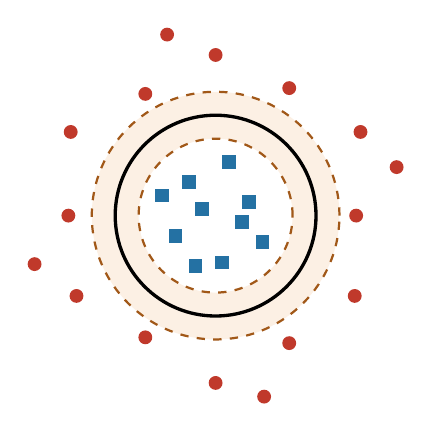
\begin{tikzpicture}[scale=0.85]
  \fill[svc!12,even odd rule] (0,0) circle (1.85) (0,0) circle (1.15);
  \draw[svc!70!black,thick,dashed] (0,0) circle (1.85);
  \draw[svc!70!black,thick,dashed] (0,0) circle (1.15);
  \draw[very thick] (0,0) circle (1.5);
  \foreach \p in {(0.5,0.2),(-0.4,0.5),(0.1,-0.7),(-0.6,-0.3),(0.7,-0.4),(0.2,0.8),(-0.2,0.1),(-0.8,0.3),(0.4,-0.1),(-0.3,-0.75)}
    \node[ptneg] at \p {};
  \foreach \a/\r in {0/2.1,30/2.5,60/2.2,90/2.4,120/2.1,150/2.5,180/2.2,210/2.4,240/2.1,270/2.5,300/2.2,330/2.4,15/2.8,105/2.8,195/2.8,285/2.8}
    \node[ptpos] at (\a:\r) {};
\end{tikzpicture}\\
\scriptsize RBF kernel: a circular boundary in the original space.
\column{0.56\textwidth}
\small
Training solves the dual with $K$, giving $\hat\alpha^{(i)}$. A new instance $\x$ is classified using \textbf{only the support vectors}:
\[
  h(\x) = \sum_{\hat\alpha^{(i)}>0}\hat\alpha^{(i)}t^{(i)}\,K\big(\x^{(i)},\x\big) + \hat b,
\]
\[
  \hat y = \begin{cases}0 & h(\x)<0\\ 1 & h(\x)\ge0\end{cases}
\]
with the bias computed from the support vectors:
\[
  \hat b = \frac{1}{n_s}\sum_{\hat\alpha^{(i)}>0}\Big(t^{(i)} - \sum_{\hat\alpha^{(j)}>0}\hat\alpha^{(j)}t^{(j)}K\big(\x^{(i)},\x^{(j)}\big)\Big).
\]
\begin{itemize}
  \item The decision boundary is \textbf{nonlinear} in the original space.
  \item $\hat\w$ is never computed, since it lives in feature space.
\end{itemize}
\end{columns}
\end{frame}

% ==================================================================
\begin{frame}{The Gaussian RBF kernel and the hyperparameter $\gamma$}
\begin{columns}[c]
\column{0.44\textwidth}
\centering
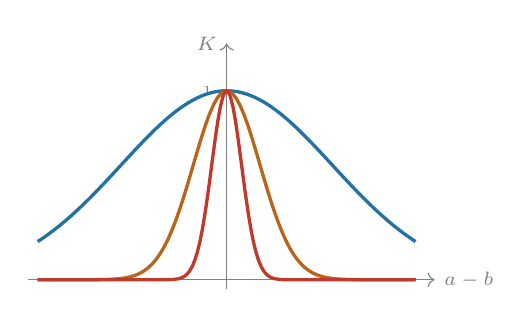
\begin{tikzpicture}[x=0.6cm,y=2.4cm]
  \draw[->,gray] (-4.2,0) -- (4.4,0) node[right] {\scriptsize $a-b$};
  \draw[->,gray] (0,-0.05) -- (0,1.25) node[left] {\scriptsize $K$};
  \draw[gray] (0.1,1) -- (-0.1,1) node[left,font=\tiny] {$1$};
  \draw[negc,very thick,domain=-4:4,samples=100] plot (\x,{exp(-0.1*\x*\x)});
  \draw[svc!80!black,very thick,domain=-4:4,samples=100] plot (\x,{exp(-1*\x*\x)});
  \draw[posc,very thick,domain=-4:4,samples=150] plot (\x,{exp(-5*\x*\x)});
\end{tikzpicture}\\[2pt]
\scriptsize 1-D example: $K(a,b)=\exp(-\gamma(a-b)^2)$\\
  {\color{negc}$\gamma=0.1$}, {\color{svc!80!black}$\gamma=1$}, {\color{posc}$\gamma=5$}
\column{0.54\textwidth}
\small
\begin{itemize}
  \item $K(\mathbf a,\mathbf b)$ is a \textbf{similarity}: $1$ when $\mathbf a=\mathbf b$, decaying to $0$ as the points move apart.
  \item $h(\x)$ is a weighted sum of ``bumps'' centered at the support vectors.
  \item \textbf{Small $\gamma$:} wide bumps, so each instance has a large range of influence. The boundary is \emph{smooth} and the model may \emph{underfit}.
  \item \textbf{Large $\gamma$:} narrow bumps. The boundary is \emph{irregular} and wiggles around individual instances, so the model may \emph{overfit}.
  \item $\gamma$ acts like a regularization hyperparameter: if the model overfits, \textbf{reduce} $\gamma$. If it underfits, increase it. Tune $\gamma$ together with $C$.
\end{itemize}
\end{columns}
\end{frame}

% ==================================================================
\begin{frame}{Which kernel and which class to use?}
\small
\begin{itemize}
  \item Always try the \textbf{linear} kernel first. \texttt{LinearSVC} is much faster than \texttt{SVC(kernel="linear")}, especially for large training sets or many features.
  \item If the training set is not too large, try the \textbf{Gaussian RBF} kernel next. It works well in most cases.
  \item Use \textbf{cross-validation and grid search} to choose the kernel and to tune $C$, $\gamma$ (and $d$).
  \item SVMs are sensitive to feature scales, so always \textbf{scale the features} first (e.g.\ \texttt{StandardScaler}).
\end{itemize}
\begin{center}
\begin{tabular}{@{}lcccc@{}}
\toprule
Class & Time complexity & Out-of-core & Scaling required & Kernel trick \\
\midrule
\texttt{LinearSVC} & $O(m\times n)$ & No & Yes & No \\
\texttt{SGDClassifier} & $O(m\times n)$ & Yes & Yes & No \\
\texttt{SVC} & $O(m^2\times n)$ to $O(m^3\times n)$ & No & Yes & Yes \\
\bottomrule
\end{tabular}
\end{center}
\vspace{2pt}
\centering\scriptsize $m$ = number of instances, $n$ = number of features. \texttt{SVC} becomes very slow for large $m$ (hundreds of thousands of instances).
\end{frame}

% ==================================================================
\begin{frame}{SVM regression: reversing the objective}
\begin{columns}[T]
\column{0.5\textwidth}
\centering
\textbf{Large $\varepsilon$} ($\varepsilon=0.6$)\\[3pt]
\svrpanel{0.6}{2.6/-0.6,3.4/0.7}
\column{0.5\textwidth}
\centering
\textbf{Small $\varepsilon$} ($\varepsilon=0.25$)\\[3pt]
\svrpanel{0.25}{0.3/0.3,0.8/-0.4,1.7/0.5,2.6/-0.6,3.4/0.7,3.9/-0.3,4.8/-0.5,5.2/0.4}
\end{columns}
\vspace{4pt}
\small
\begin{itemize}
  \item \textbf{Classification:} fit the widest street with \emph{no} instances inside it.
  \item \alert{Regression:} fit a street of width $2\varepsilon$ with as many instances as possible \emph{inside} it, while limiting the instances that fall outside.
  \item The model is \textbf{$\varepsilon$-insensitive}: adding training instances inside the street does not change the predictions. Only instances on or outside the street (circled) are \textbf{support vectors}.
\end{itemize}
\end{frame}

% ==================================================================
\begin{frame}{Linear SVM regression: the optimization problem}
\begin{columns}[c]
\column{0.62\textwidth}
\small
With prediction $h(\x)=\w^\top\x+b$ and real-valued targets $y^{(i)}$:
\begin{alertblock}{Linear SVR objective}
\[
  \underset{\w,b,\bm\zeta,\bm\zeta^*}{\text{minimize}}\quad
  \frac12\w^\top\w + C\sum_{i=1}^{m}\big(\zeta^{(i)}+\zeta^{*(i)}\big)
\]
\vspace{-6pt}
\[
  \text{s.t.}\quad
  \begin{aligned}
    y^{(i)} - h(\x^{(i)}) &\le \varepsilon + \zeta^{(i)} && \text{(above the street)}\\
    h(\x^{(i)}) - y^{(i)} &\le \varepsilon + \zeta^{*(i)} && \text{(below the street)}\\
    \zeta^{(i)},\ \zeta^{*(i)} &\ge 0 .
  \end{aligned}
\]
\end{alertblock}
Equivalently, minimize $\frac12\w^\top\w + C\sum_i L_\varepsilon\big(y^{(i)}-h(\x^{(i)})\big)$ with the \textbf{$\varepsilon$-insensitive loss}
\[
  L_\varepsilon(r) = \max\big(0,\ |r|-\varepsilon\big).
\]
\column{0.36\textwidth}
\centering
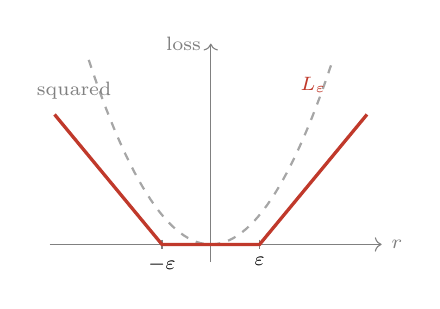
\begin{tikzpicture}[x=0.62cm,y=0.75cm]
  \draw[->,gray] (-3.3,0) -- (3.5,0) node[right] {\scriptsize $r$};
  \draw[->,gray] (0,-0.3) -- (0,3.4) node[left] {\scriptsize loss};
  \foreach \xx in {-1,1} \draw[gray] (\xx,0.08) -- (\xx,-0.08);
  \node[below,font=\scriptsize] at (-1,-0.05) {$-\varepsilon$};
  \node[below,font=\scriptsize] at (1,-0.05) {$\varepsilon$};
  \draw[gray!70,thick,dashed,domain=-2.5:2.5,samples=60] plot (\x,{0.5*\x*\x});
  \draw[posc,very thick] (-3.2,2.2) -- (-1,0) -- (1,0) -- (3.2,2.2);
  \node[posc,font=\scriptsize,align=center] at (2.1,2.7) {$L_\varepsilon$};
  \node[gray,font=\scriptsize] at (-2.8,2.6) {squared};
\end{tikzpicture}\\
\scriptsize Errors smaller than $\varepsilon$ cost nothing. Larger errors cost \emph{linearly}, so the model is robust to outliers.
\end{columns}
\end{frame}

% ==================================================================
\begin{frame}{Nonlinear SVM regression}
\begin{columns}[c]
\column{0.42\textwidth}
\centering
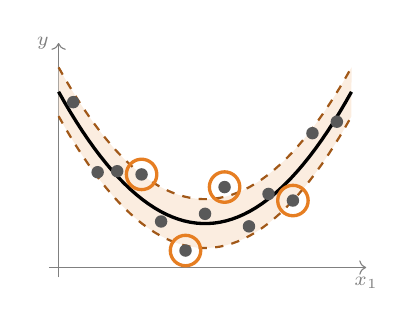
\begin{tikzpicture}[scale=0.62]
  \draw[->,gray] (-0.2,0) -- (6.3,0) node[below] {\scriptsize $x_1$};
  \draw[->,gray] (0,-0.2) -- (0,4.6) node[left] {\scriptsize $y$};
  \fill[svc!14,domain=0:6,samples=50] plot (\x,{0.3*(\x-3)^2+0.9-0.5}) -- plot[domain=6:0] (\x,{0.3*(\x-3)^2+0.9+0.5}) -- cycle;
  \draw[svc!70!black,thick,dashed,domain=0:6,samples=50] plot (\x,{0.3*(\x-3)^2+0.9-0.5});
  \draw[svc!70!black,thick,dashed,domain=0:6,samples=50] plot (\x,{0.3*(\x-3)^2+0.9+0.5});
  \draw[very thick,domain=0:6,samples=50] plot (\x,{0.3*(\x-3)^2+0.9});
  \foreach \xx/\nn in \regnoise \node[ptreg] at (\xx,{0.3*(\xx-3)^2+0.9+\nn}) {};
  \foreach \xx/\nn in {2.6/-0.6,3.4/0.7,4.8/-0.5,1.7/0.5} \node[sv] at (\xx,{0.3*(\xx-3)^2+0.9+\nn}) {};
\end{tikzpicture}\\
\scriptsize 2nd-degree polynomial kernel, $\varepsilon=0.5$.
\column{0.56\textwidth}
\small
Apply the \textbf{kernel trick} to the dual of the SVR problem. The prediction becomes
\[
  h(\x) = \sum_{i\in\text{SV}}\big(\hat\alpha^{(i)}-\hat\alpha^{*(i)}\big)\,K\big(\x^{(i)},\x\big) + \hat b .
\]
\textbf{Hyperparameters:}
\begin{itemize}
  \item $\varepsilon$: width of the street. A larger $\varepsilon$ gives fewer support vectors and a simpler model.
  \item $C$: penalty for instances outside the street. A smaller $C$ gives more regularization.
  \item Kernel and its parameters ($d$, $\gamma$, \dots).
\end{itemize}
\textbf{Scikit-Learn:}\\[2pt]
\scriptsize
\texttt{LinearSVR(epsilon=0.5)}\\
\texttt{SVR(kernel="poly", degree=2, C=100, epsilon=0.1)}\\
\small
Scaling and complexity: as for \texttt{LinearSVC} and \texttt{SVC}.
\end{columns}
\end{frame}

% ==================================================================
\begin{frame}{Summary}
\small
\begin{columns}[T]
\column{0.49\textwidth}
\begin{itemize}
  \item \textbf{Large margin classification:} among all separating hyperplanes, choose the one with the widest street. The street is determined only by the \textbf{support vectors}.
  \item \textbf{Hard margin:} $\min \tfrac12\w^\top\w$ \ s.t.\ $t^{(i)}(\w^\top\x^{(i)}+b)\ge1$. Requires linearly separable data and is sensitive to outliers.
  \item \textbf{Soft margin:} add slack variables $\zeta^{(i)}$ and the penalty $C\sum_i\zeta^{(i)}$, which is equivalent to the hinge loss. $C$ trades street width against violations: if the model overfits, reduce $C$.
\end{itemize}
\column{0.49\textwidth}
\begin{itemize}
  \item \textbf{Kernel trick:} the dual uses data only through dot products. Replacing them by $K(\mathbf a,\mathbf b)=\phi(\mathbf a)^\top\phi(\mathbf b)$ gives nonlinear boundaries without computing $\phi$.
  \item \textbf{Kernels:} linear, polynomial, Gaussian RBF (tune $\gamma$: if overfitting, reduce it), sigmoid.
  \item \textbf{SVM regression:} fit as many instances as possible \emph{inside} a street of width $2\varepsilon$, using the $\varepsilon$-insensitive loss.
\end{itemize}
\end{columns}
\begin{alertblock}{In practice}
Scale the features $\;\to\;$ try \texttt{LinearSVC}/\texttt{LinearSVR} first $\;\to\;$ then \texttt{SVC}/\texttt{SVR} with an RBF kernel $\;\to\;$ tune $C$, $\gamma$ (and $\varepsilon$) with cross-validation.
\end{alertblock}
\end{frame}

\end{document}
